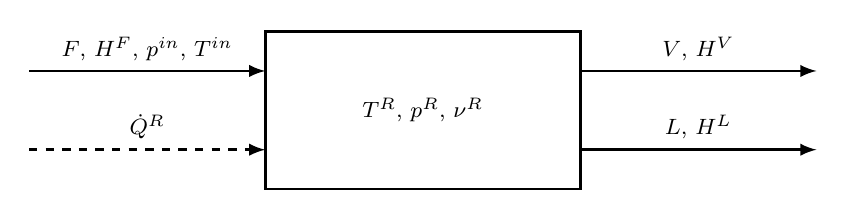
\begin{tikzpicture}[arrow/.style={line width=1pt,->,>=latex}]
	\draw [line width=1pt] (-2,2) rectangle (2,0) node at (0,1) {\footnotesize $T^R$, $p^R$, $\nu^R$};
	\draw [arrow] (-5,1.5) -- (-2,1.5) node [pos=0.5, above] {\footnotesize $F$, $H^F$, $p^{in}$, $T^{in}$};
	\draw [line width=1pt,->,>=latex,dashed] (-5,0.5) -- (-2,0.5) node [pos=0.5, above] {\footnotesize $\dot{Q}^R$};
	\draw [arrow] (2,1.5) -- (5,1.5) node [pos=0.5, above] {\footnotesize $V$, $H^V$};
	\draw [arrow] (2,0.5) -- (5,0.5) node [pos=0.5, above] {\footnotesize $L$, $H^L$};
\end{tikzpicture}�